\documentclass[12pt]{article}
\usepackage[a4paper, margin=2cm]{geometry}
\usepackage[english]{babel} % To obtain English text with the blindtext package
\usepackage{blindtext}
\usepackage{graphicx} % Required for inserting images
\usepackage{array, multirow} % For extra column formatting
\usepackage{amsmath, amssymb, cancel} %for equation environment
\usepackage{float}
\usepackage{parskip} % For gaps between para
\usepackage{setspace}
\usepackage{pdfpages}
\usepackage{abstract}
\usepackage{longtable}
\usepackage[export]{adjustbox}
\usepackage{emptypage}
\usepackage{tocloft}
\usepackage[nottoc]{tocbibind}
\usepackage{hyperref, url}
\usepackage[table]{xcolor}
\usepackage{minted}
    \usemintedstyle{monokai}
\usepackage{caption}
    \captionsetup{font=footnotesize,labelfont=bf}
\usepackage{tcolorbox}
    \newtcolorbox{mintedbox}{
        colback=backcolour,
        boxrule=0pt,
        sharp corners,
        width=\linewidth,
        left=0pt, right=0pt,
        top=3pt, bottom=3pt
    }

\cftsetindents{section}{0em}{2em}
\cftsetindents{subsection}{0em}{2em}

\renewcommand\cfttoctitlefont{\hfill\Large\bfseries}
\renewcommand\cftaftertoctitle{\hfill\mbox{}}

\graphicspath{ {./images/} }

\pagenumbering{arabic}

\definecolor{blurple}{HTML}{5865F2}
\definecolor{backcolour}{HTML}{272823}

\hypersetup{
    colorlinks=true,
    linkcolor=black,
    urlcolor=blurple,
    citecolor=blurple,
}

\urlstyle{same}

\renewcommand{\arraystretch}{1.3}

\setcounter{secnumdepth}{5}
\setcounter{tocdepth}{5}
\newcommand\simpleparagraph[1]{%
  \stepcounter{paragraph}\paragraph*{\theparagraph\quad{}#1}}

%%%%%%%%%%%%%%%%%%%%%%%%%%%%%%%%%%%


\title{PHYC20040 Exp.2 Pleiades SM}
\author{Joana Adao}
\date{\today}

\begin{document}

\begin{titlepage}
    \begin{center}

        \begin{figure}[ht]
            
\includegraphics[width=\textwidth]{UCDLogo.png}
        \end{figure}
        
        \begin{figure}
            \centerline{
\includegraphics[width=\paperwidth]{UCDBanner.png}}
        \end{figure}

        \vspace{4cm}

        {\LARGE \bfseries PHYC20040 Exploring the Solar System}\\
        \vspace{0.75cm}
        {\Large Experiment No.3 The Classification of Stellar Spectra}
        
        \vspace{1cm}
    
    {\Large \textbf{26 February 2025}}

    \vspace{2cm}
    
    {\large \textbf{by Joana C.C. Adao (Student No. 23311051)}}\\

    \end{center}
    
   \clearpage

\end{titlepage}

\setcounter{page}{1}
\tableofcontents

\newpage

\begin{abstract}
\addcontentsline{toc}{section}{Abstract}



\end{abstract}

%%%%%%%%%%%%%%%%%%%%%%%%%%%%%%%%%%%

\vspace{4cm}

\section{Theory} \label{sec:1}

\subsection{Spectra}

The electromagnetic spectrum describes all forms of electromagnetic radiation, including visible light, as it varies with wavelength
and frequency  
\cite{britspectra,hubblespectra}.
Spectroscopes are equipments used to visually observe the spectra and spectrographs photograph and map the studied spectra
\cite{britspectra}.
There are three main ways that the spectra can be classified, as illustrated in figure \ref{fig:spectra} \cite{spectrapic}.

\begin{figure}[H]
    \centering
    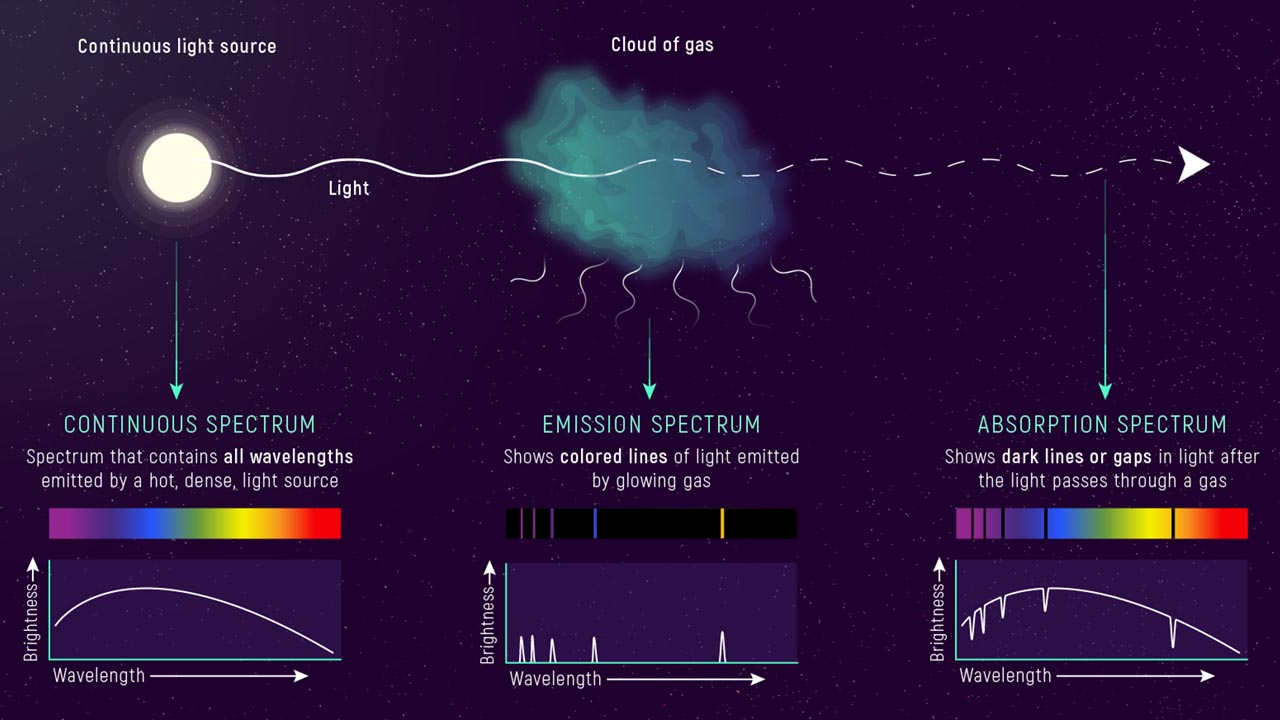
\includegraphics[width=15cm]{spectra.jpg}
    \caption{\centering \footnotesize{Types of spectra: continuous, emission, absorption \protect\cite{spectrapic}}}
    \label{fig:spectra}
\end{figure}

\textbf{Spectrometry} puts quantitative values to the theory explored by spectroscopy (\textit{theoretical} interaction between radiation and matter) by measuring the interactions between light (electromagnetic radiation)
and matter
\cite{ataspectrosco}.

\subsubsection{Absorption Line Spectra}

\textbf{The absorption spectrum} is measured when light from a continuous source, like a star, passes through a cloud of cooler gas.
The wavelengths that will be absorbed depend on the composition and elements of the gas, as well as its temperature and density. The wavelengths
that didn't pass through are what appear as dark lines on the continuous spectrum known as the absorption line spectrum \cite{cosmosabsorp}.

\subsubsection{Emission Line Spectra}

\textbf{The emmission spectrum} is measured when atoms become excited after light, like from a star, passes through a cloud of gas.
The light can heat up the cloud of gas, thus exciting the atoms and causing them to release light. The light which the gas releases depends on the
composition and elements, temperature, and density of the gas cloud. The light emitted will appear as coloured lines.

\subsection{Blackbody Radiation} \label{sec:1.1}

Blackbodies are idealised surfaces that can absorb any wavelenght of incident radiation without any reflection, and that can emit electromagnetic (EM) radiation
at maximum possible monochomatic intensities for a range of wavelengths (a continuous spectrum) based on temperature
\cite{librablackodyrad,UCDblackbocdyrad,ESAblackbodyrad}.

\begin{figure}[H]
    \centering
    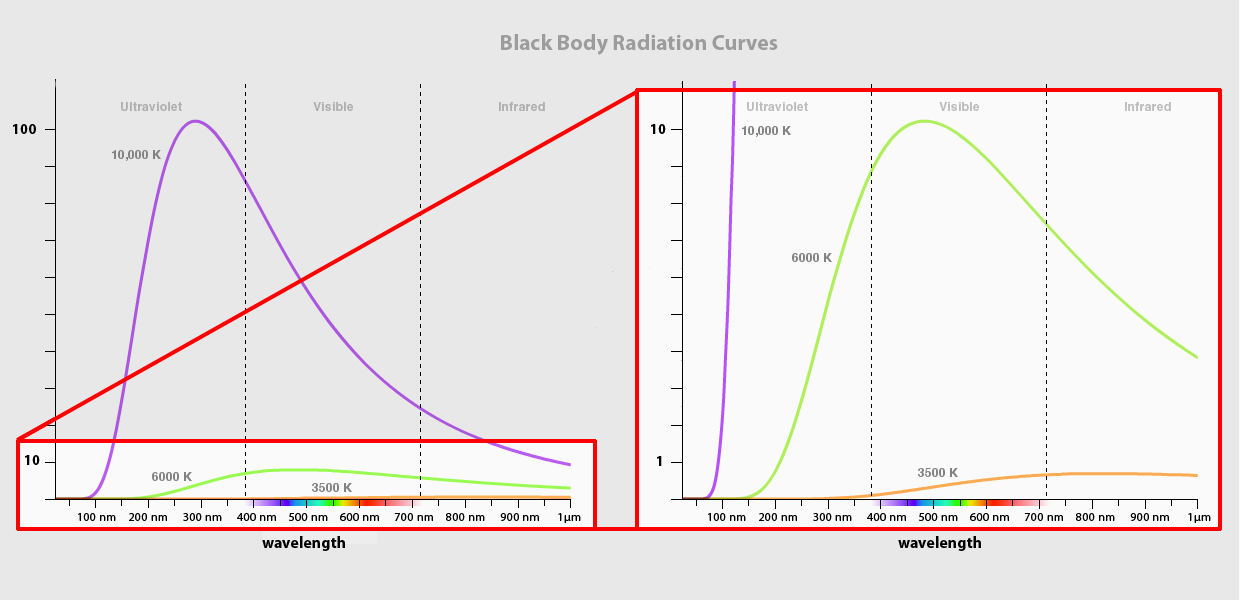
\includegraphics[width=12.5cm]{blackbody.jpg}
    \caption{\centering Diagram of blackbody radiation curves for stars of 10 000K, 6 000K, 3 500K, with the visible light spectrum shown on the x-axis \protect\cite{ESAblackbodyrad}.}
    \label{fig:blackbodyrad}
\end{figure}

The characteristic curve of the continuous spectrum of blackbody radiation can be used to determine the temperatures of stars and other cosmic objects by finding their "colour" \cite{ESAblackbodyrad}.
Hotter stars emit shorter wavelengths and therefore appear bluer, while colder stars emit longer wavelengths and therefore appear redder (see figure \ref{fig:msgraphspec}).


\subsection{Wien's Displacement Law}

Wien's Law relates the peak wavelength of a blackbody's peak emission spectrum ($\mathbf{\lambda_{peak}}$) to temperature (\textbf{T}) \cite{derivwien}.
This is given by the following, with $\mathbf{\lambda_{peak}}$ in metres (m) and temperature \textbf{T} in Kelvin (K) \cite{derivwien}:

\vspace{-1.5ex}
\begin{gather}
    \lambda_{peak} (\text{m}) = \frac{2.89777 \times 10 ^{-3}}{T} 
\end{gather}

The wavelength $\mathbf{\lambda_{peak}}$ can also be found in Ångstroms (Å) by changing the numerator constant to be in Ångstrom-Kelvin instead of metre-Kelvin:

\vspace{-1.5ex}
\begin{gather}
    \lambda_{peak} (\text{\AA}) = \frac{2.9 \times 10^7}{T}
\end{gather}

\subsection{Apparent and Absolute Magnitude} \label{sec:1.1.3}

Magnitude is a logarithmic measure of the brightness of a star or other celestial body. The brighter the object, the lower the magnitude (number), and they can be negative for particularly bright stars
\cite{britmag}.
The magnitude of the celestial objects are divided into two types of observation:

\begin{itemize}
    \item \textbf{Apparent magnitude, m,} is used to describe how bright a celestial object appears from the view on Earth
    \cite{lcomag}.
    \item \textbf{Absolute magnitude, M,} also in reference to \textbf{\textit{luminosity}}, is defined as the magnitude of the star if the distance between it and Earth were 10 parsecs (pc)
    \cite{lcoabsmag,cosmosabsmag}.
    When at a set distance, astronomers are then able to compare intrinsic brightness of stars
    \cite{cosmosabsmag}.
\end{itemize}

Absolute (\textbf{M}) and apparent (\textbf{m}) magnitudes can be used in equation \ref{eq:1} to calculate \textbf{D}, the distance in parsecs (pc).
The distance modulus is then $\mathbf{m - M}$.  The magnitudes do not have units
\cite{cosmosabsmag}.

\vspace{-1.5ex}
\begin{gather} \label{eq:1}
    M = m + 5 - 5 (\log_{10} D) \quad , \quad m - M = 5 \log_{10} \left( \frac{D}{10} \right)
\end{gather}

The above equation (\ref{eq:1}) can then be manipulated to find the distance, \textbf{D}:

\vspace{-1.5ex}
\begin{gather} \label{eq:2}
    \log_{10}D = \frac{m - M + 5}{5} \quad \implies \quad D = 10^{\frac{m - M + 5}{5}}
\end{gather}

\subsection{Stellar Classification}

\subsubsection{Harvard Classification of Spectral Types} \label{sec:1.2.1}

The currently-used system of classification of stars was created by a team at Harvard in 1924 \cite{harvardstar}. The different classes are \textbf{OBAFGKM}, left to right: hottest to coolest.
The different classes and temperature thresholds are illustrated in figure \ref{fig:starclassy}.

\begin{figure}[H]
    \centering
    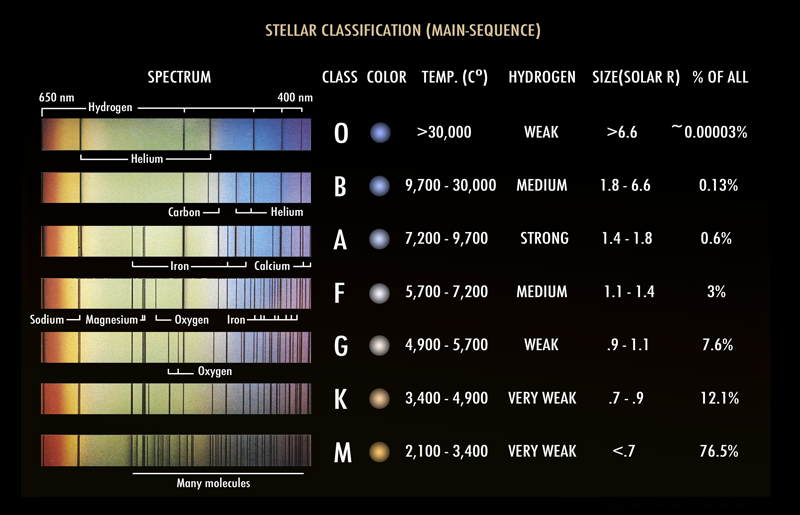
\includegraphics[width=.9\textwidth]{Stellar_Classification_Chart.png}
    \caption{\centering Chart for classifying of the main star types as per the Harvard classification \protect\cite{wikistar}.}
    \label{fig:starclassy}
\end{figure}

Subclasses of numbers ranging from 0-9 allow for finer distinctions in temperature within the OBAFGKM classes. 
For example, the Sun is spectral type \textbf{G2} with a temperature of about 5 700 K (Kelvin) \cite{cosmosstar}.

\subsubsection{MK System of Luminosity}

The Morgan-Keega (MK) Luminosity Class is an addition to the Harvard stellar classification scheme (see §\ref{sec:1.2.1}), given in the form of (primarily) Roman numerals.
This addition to the system was devised in order to be able to distinguish between stars of similar temperatures but differing \textit{luminosities}.

The MK System was originally from I to V, but has since been expanded to differentiate more between I-type stars and further beyond V.
The table containing the luminosity classifications is shown below \cite{mkcosmos}:

\begin{table}[H]
    \centering
    \caption{Table of the MK Luminosity Classes \protect\cite{mkcosmos}.}
    \begin{tabular}{
    |>{\columncolor[HTML]{EFEFEF}}c| c|}
    \hline
    \textbf{Class} & \textbf{Star Type}             \\ \hline
    Ia-O           & extremely luminous supergiants \\
    Ia             & luminous supergiants           \\
    Ib             & less luminous supergiants      \\
    II             & bright giants                  \\
    III            & normal giants                  \\
    IV             & subgiants                      \\
    V              & main sequence dwarf stars      \\
    VI, or sd      & subdwarfs                      \\
    D              & white dwarfs                   \\ \hline            
    \end{tabular}
    \label{tab:1}
\end{table}

\subsubsection{Main Sequence Stars} \label{sec:1.2.2}

Main sequence stars have nuclear reactions at their core through the fusion of hydrogen atoms into helium that allow them to sustain themselves
\cite{schoolmsstar,studymsstar,nasamsstar}.
The radiation pressure from the nuclear reactions and the gravitational pressure work against each other in such a way that the star
remains stable \cite{studymsstar} in a process known as \textbf{hydrostatic equilibrium} \cite{schoolmsstar}.

Figure \ref{fig:msgraphspec} shows the graph of the absorption line spectrum for specific main sequence stars ranging from A to M, excluding classes B and O.

\begin{figure}[H]
    \centering
    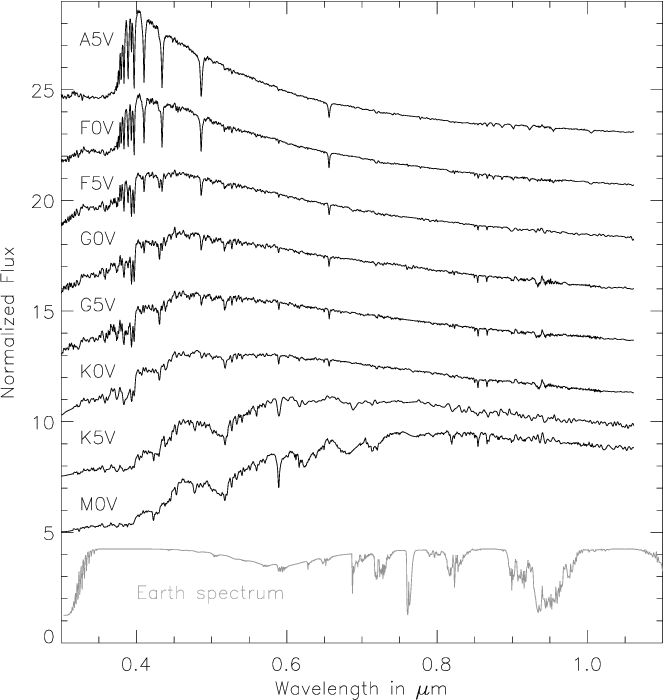
\includegraphics[width=12.5cm]{msspectra.png}
    \caption{\centering Stellar spectra of the main sequence (V) stars (A5 to M0) \protect\cite{msspectrarticle}.}
    \label{fig:msgraphspec}
\end{figure}

\section{Methodology} \label{sec:2}



\section{Results and Calculations} \label{sec:3}



\newpage

\section{Conclusion} \label{sec:4}



\newpage

%%%%%%%%%%%%%%%%%%%%%%%%%%%%%%%%%%%

\bibliographystyle{IEEEtran}
\bibliography{References} \label{sec:ref}

\vspace{1.5cm}

\listoffigures

\listoftables

\section*{Appendix} \label{sec:A}
\addcontentsline{toc}{section}{Appendix}

\subsection*{Tables}
\addcontentsline{toc}{subsection}{Tables}



\subsection*{Graphs}
\addcontentsline{toc}{subsection}{Graphs}



\subsection*{Code}
\addcontentsline{toc}{subsection}{Code}

%

\begin{minipage}{\linewidth}
\captionsetup{hypcap=false}

\begin{mintedbox}
\begin{minted}[fontsize=\small, breaklines, baselinestretch=1.2, xleftmargin=0.5cm]{python}
import numpy as np
import matplotlib.pyplot as plt


\end{minted}
\end{mintedbox}

\captionof{figure}{\centering Code}
\end{minipage}


\end{document}